% -*-latex-*-
%
%  The contents of this file are subject to the University of Utah Public
%  License (the "License"); you may not use this file except in compliance
%  with the License.
%
%  Software distributed under the License is distributed on an "AS IS"
%  basis, WITHOUT WARRANTY OF ANY KIND, either express or implied. See the
%  License for the specific language governing rights and limitations under
%  the License.
%
%  The Original Source Code is SCIRun, released March 12, 2001.
%
%  The Original Source Code was developed by the University of Utah.
%  Portions created by UNIVERSITY are Copyright (C) 2001, 1994
%  University of Utah. All Rights Reserved.
%

\section{Concepts}
\label{sec:concepts} 
\index{concepts}

This section describes the general design philosphy and goals of
integrated problem solving environments \index{problem solving
  environment} and how \BIOPSE{} embodies some of these ideas.

\subsection{Traditional problem solving methods}

The traditional method for solving bioelectric field problems uses
multiple, non-integrated computer programs.  For example, a scientist using
a computer simulation to examine the effect of electrode patch placement on
transcardiac current density in the design of a cardiac implantable
defibrillator\cite{CRJ:Sch95b} would require geometric modeling, numerical
simulation, and scientific visualization tools to complete the task.  The
user might need one program to define the thoracic surfaces from medical
images and another to create a discrete mesh of the volume contained within
the surfaces\cite{CRJ:Sch93b}.  Another application like Matlab computes a
finite element simulation of the electric current distribution from the
defibrillation electrodes through the thoracic volume\cite{RSM:And93}.
Another approach might be to write a Fortran program using a public domain
numerical library such as LAPACK\@ \index{LAPACK}.  To see the output would
require a scientific visualization package (such as those described
in\cite{RSM:All91}).  Between each of these steps, it would be necessary to
save the output of one program in a format that the next in the sequence
could read---this would usually necessitate separate file format conversion
utilities.  To find the optimal location, shape, and size parameters for
the defibrillating electrode, the scientist would have to go back to the
geometric modeling package, change the necessary parameters, manually
re-run all of the subsequent steps to see how the new electrode
configuration affects the current density distribution, and then manually
iterate.  The manual intervention required to drive this process is both
tedious and time consuming.

Far more efficient is a scenario in which the user could define an
appropriate set of parameters for a given simulation, and then set up
a sequence of runs to examine each of them and save the results for
subsequent examinations.  The complete execution of the sequence might
require hours or even days, but the user would be free during that
time to perform other tasks.  This process is similar to the ``what
if?'' analysis that modern spreadsheet programs offer for much simpler
problems.  

In our example of the defibrillation simulation, the scientist could
select various locations and orientations for the defibrillation
electrodes, choose values for the other parameters of the simulation
(\eg{} the number of nodes in the finite element model, the boundary
conditions, the error tolerance for convergence, and the evaluation
criteria), and leave the simulations to run as long as necessary.
Viewing the results could be as simple as watching the animation
produced by the simulation or scanning other defibrillation quality
indices such as maximum and minimum current density magnitude or
current density histograms from the heart.  This automated execution
process, whereby the user selects all of the parameters in advance and
does not control the intra- or inter-package execution is called
\emph{batch processing}.  A primary benefit of batch processing is
that it allows the scientist to utilize computational resources
without intervention.  However, most scientific computer software
demands (or requires) at least some user intervention in order to
produce meaningful results .  This constraint makes it difficult or
impossible to run multiple computational jobs automatically, leaving
the user with the task of manually initiating and controlling each
step of the process.

\subsection{Integrated problem solving and computational
steering} 
\label{sec:con-steering} 

The goal of integrated problem solving environments---and specifically
of \SR{} and \BIOPSE{}---is to incorporate and integrate all the steps
described in the previous example as components in a single, unified,
extensible problem solving environment \index{PSE}.  The functionality
that will result includes the ability to manage each step in a
sequential computing process, and to create batch processes that
execute repeated simulations.  However, the functionality that sets
\SR{} and \BIOPSE{} apart from most integrated software environments
is the ability to intervene and control execution anywhere in the
chain at any time during its execution.  This ability to control a
computer program during execution is termed \emph{computational
  steering.}

To provide a non-technical analogy, adding computational steering to a
software environment is similar to adding the ability to occasionally
switch tracks in train travel.  A train passenger can get on the train
and automatically get to a new destination, leaving all the details of
the individual actions to the rail system machinery and staff.  But
the route and the destination are fixed.  Steering would permit each
passenger to request that the train take a new route, with different
stops, and even a different destination, and be able to make these
decisions at any time during the trip.  In the more rigorous example
of the defibrillation simulation, computational steering allows a
scientist to interactively change parameters and settings as the
simulation executes, performing his work both in batch and interactive
modes.  Steering interventions might include adjusting electrode
locations to stay within anatomically reasonable bounds or refining
the geometric model resolution in order to balance accuracy and
execution time.

To achieve integration within the elements of \SR{} and \BIOPSE{},
data flows directly from one processing step to the next, without ever
being diverted to a disk file or leaving the program.  Output from
each step is available as input to dependent steps.  The underlying
paradigm of \SR{} is of data flowing between modules that each perform
some operation.  Integration between modules guarantees that upon
completion of their tasks, upstream modules pass their data to
downstream modules, thereby forcing the downstream modules to execute
in response.  In our example, this means that the scientist may alter
electrode locations at any time, thus initiating a sequence of all the
necessary steps to recompute the simulation with the new
configuration.  The modification of the geometric model, finite
element calculation, and visualization all proceed automatically and
in the proper sequence, all managed by \SR{}.  This combination of
steering and component integration allows the scientist to
spontaneously explore a problem.

While computational steering is still a young field in computer
science, there are a number of examples of such systems (in addition
to \SR{}) described in the literature.  Burnett\cite{MM:Bur94}, and
Vetter and Schwan\cite{MM:Vet96} give overviews of existing
computational steering system.  Several notable examples include
CUMULVS\cite{MM:Gei96,MM:Koh97}, \index{CUMULVS}
Progress\cite{MM:Vet95}, \index{Progress} and Magellan\cite{MM:Vet97a}
\index{Magellan}.



\subsubsection{\SR{} and its Packages}
\label{sec:srversuspse}

%begin{latexonly}
\newcommand{\eabfig}{%
  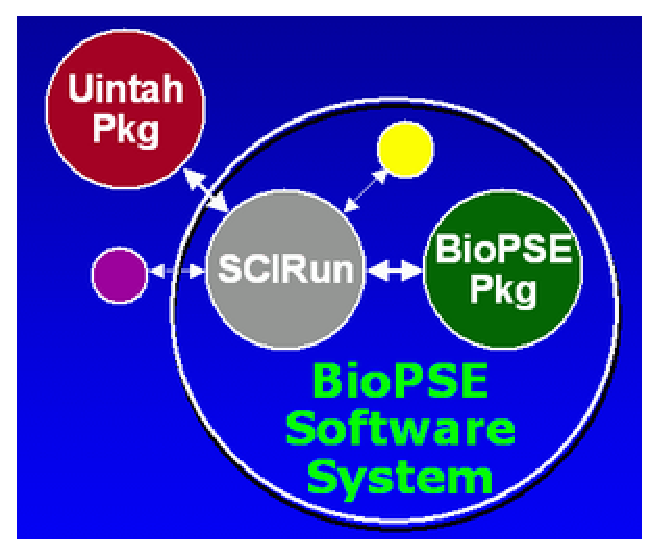
\includegraphics{../FAQ/EAB-BioPSE.eps}
}
%end{latexonly}
\begin{htmlonly}
  \newcommand{\eabfig}{%
    \htmladdimg[align=left,alt=""]{../../FAQ/EAB-BioPSE.gif}
  }
\end{htmlonly}

It is important to understand the place of the software included in
this package within the hierarchy of computational problem solving
environments developed at the SCI Institute.  From a historical
perspective, \SR{}, which we started developing in 1992, was the
original implementation of the computational
framework\cite{CRJ:Joh94c,RSM:Par95,RSM:Par95b,RSM:Par97,RSM:Par97b,CRJ:Parker99b}.
Since then, \SR{} and its computational workbench infrastructure have
been the basis of many significant application-specific projects.  Two
major examples are the DOE sponsored Uintah system \cite{RSM:Dav2000}
and the NIH sponsored \BIOPSE{} system.  The target applications of
the Uintah project are combustion, computational fluid dynamics, and
mechanical modeling implemented on large-scale, distributed, shared
memory architectures.  The goal of the \BIOPSE{} project is to create
software for geometric modeling, simulation, and visualization for
solving bioelectric field problems.  An important secondary goal of
the \SR{} system is to make source code for these problem solving
environments publicly available to the scientific community.

\begin{figure}[htb]
  \centering
  \begin{makeimage} \end{makeimage}
  \eabfig
  \caption{\label{fig:eab-BioPSE} \sr{} and its relation to its
    packages.  BioPSE (for example) consists of the basic \sr{}
    software together with the BioPSE modules and support libraries.}
\end{figure}

To realize these two significant projects, the \SR{} infrastructure
itself has required significant reorganization, extension, and
enhancement.  Even with these recent changes, \SR{} remains both the
core infrastructure for our problem solving environments and the name
we use to refer to the entire ensemble of software.  Thus a user may
install and operate the core \SR{} software and also augment its
functionality with one or more of its packages such as \BIOPSE{} as
shown in Figure~\ref{fig:eab-BioPSE}.  We anticipate that the
collection of packages will grow as the advantages of the \SR{}
infrastructure become available to scientists and engineers of all
disciplines.

In addition to the major projects that have both leveraged and
advanced \SR{}, there exist a number of smaller packages that extend
\SR{}'s utility.  Examples include the Teem package for raster data
processing, the NetSolve package for linear algebra subroutines
(developed by researchers at the University of Tennessee and
Knoxville), and a communications interface to the Matlab program.  We
have developed various forms of software wrappers or interfaces that
allow \SR{} to leverage the strengths of these third party tools,
links we refer to as "bridges."

There are also instances in which a tighter level of integration than a
bridge between \SR{} and third-party software is necessary.  One example
is the addition of mpeg support for capturing animations from the \SR{}
Viewer module, for which we use the Berkeley and Alex Knowles' mpeg
encoding tools.  Another example is the set of image generation and
manipulation tools from Peter Haeberli called libimage.  To indicate
whether or not such tools are available, the configure scripts for \SR{}
contain optional control flags.

We believe that this combination of a robust infrastructure and modular
extensibility through packages and third-party libraries will allow \SR{}
to grow and adapt to changing needs and opportunities. 

In this manual, we will try and be consistent about the usage of the two
terms, \SR{} and \BIOPSE{}.  \SR{} will typically refer to some feature that
is common to the core functionality of the system and this is common to all
of the problem solving environment application packages.  \BIOPSE{} will
refer to specific elements of the bioelectric field problem solving
environment.


\subsection{\SR{} Modules and Networks}
\label{sec:con-modules} 

%begin{latexonly}
  \newcommand{\basicmodule}%
  {\centerline{\epsfig{file=Figures/biopse-modmap.eps.gz,width=\columnwidth,
  bbllx=7, bblly=-193, bburx=774, bbury=14}}}
%end{latexonly}
\begin{htmlonly}
  \newcommand{\basicmodule}{%
  \htmladdimg[align=top,width=766,alt="module"]
  {../Figures/biopse-modmap.gif}}
\end{htmlonly}

The functional unit of a dataflow environment is the {\em\/module}
\index{module}.  Figure~\ref{fig:conc-module} contains a generic \SR{}
module, with a User Interface (UI) button for graphically accessing the
module's user interface, and input and output ports for receiving and sending
data, respectively.  On the right is a simple example of a dataflow
network.  Data passes through the output port of the top module, through
the data pipe, and into the input port of the bottom module.  The User
Interface enables the selection of a desired isochrone surface.

\begin{figure}[htb]
  \begin{makeimage}
  \end{makeimage}
  \basicmodule
%  \centerline{\epsfig{file=Figures/biopse-modmap.eps,width=6in}}
  \caption{\label{fig:conc-module} Example of a \SR{} module}
\end{figure}

Modules may contain other elements, but they will all have at least one
input or one output port.  Examples of a module with only an output port
would be file readers.  The \htmladdnormallink{\emph{Viewer}}{viewer.html}
module contains only input ports because it receives information and the
``output'' is a visualization.  For a more detailed description of modules and
how to control them, see \secref{Working with Networks}{sec:workwithnets}.
The most important goal at this stage is to appreciate the concept of a
module and the dataflow that links one module to another.

A network diagram \index{network!diagram} describes the way data flows
through \SR{} and is the main means of user interaction with the overall
action of the program.  The network essentially defines the basic function of
the program; without a network, \SR{} and \BIOPSE{} are just a set of tools
sitting in a chest.  By joining the modules into a network, the tools
become a functioning program that does whatever the network tells it to.
Once again, the important thing to appreciate is what the network is
conceptually; for the details, see \secref{Working with
Networks}{sec:workwithnets}. 


\subsection{\sr{}'s Use of Third Party Software}
\label{sec:con-links} 

\SR{} works together with software from third party sources in several
ways.  If you have installed \SR{} and \BIOPSE{} yourself, you will
have seen the need for third party software libraries.  The use of
third party software is largely invisible to the user of \SR{} or
\BIOPSE{}.

For example \sr{}'s user interface is written in the Tcl language
using the Tk library.  In general \sr{}'s modules use Tcl for their
user interface elements and C++ for their computations.  However, a
module may also interact with code written in other languages such as
FORTRAN or Matlab.

One of the goals of the \BIOPSE{} project is to provide
support for such external code, including FORTRAN, C, Matlab, and
IDL\@.

\subsubsection{Matlab}
\label{sec:concept-matlab} 

The interface (based on Berkeley sockets) between \SR{} and Matlab provides
a pathway to send matrix data objects from \SR{} to Matlab and then accept
the result of some Matlab computations.  At present, this arrangement
requires that a Matlab script exist that will perform the desired
operations.  \SR{} sends the input data to an existing process running
Matlab, which serves as a compute engine, performs the steps
described in the script, and then returns data to \SR{} for further
processing or display.  The Matlab process can even run on a separate
computer connected via a network, which helps to distribute the load as
well as to resolve potential licensing conflicts with Matlab.

The underlying mechanism for this communication is a socket interface
consisting of two \SR{} Modules, \module{MatrixSend} and
\module{MatrixReceive}, and a Matlab ``transport'' routine.  Both the \SR{}
and the Matlab process know about each other's whereabouts (in the form
hostname:port) and use a client-to-client communication model, so that
synchronization between processes is manual.  For example, 
the \SR{} \module{MatrixSend} module sends the matrix to a socket at which a 
Matlab script is listening.  The script then receives the matrix, 
performs the calculations in Matlab and sends the results to a socket 
where \module{MatrixReceive} module is listening.  \SR then carries out
further calculations and display of the results.

%For examples of this interface, see \secref{Matlab
%Examples}{sec:examples-matlab}.

\subsubsection{GENESIS (via SQL)}

\htmladdnormallink{GENESIS}{http://www.bbb.caltech.edu/GENESIS/genesis.html}
(short for GEneral NEural SImulation System) is a general purpose
simulation platform which was developed to support the simulation of neural
systems ranging from complex models of single neurons to simulations of
large networks made up of more abstract neuronal components. GENESIS has
provided the basis for laboratory courses in neural simulation at both
Caltech and the Marine Biological Laboratory in Woods Hole, MA, as well as
many other institutions.   

We have created a bridge between \SR{} and GENESIS so that it is possible
to use the output of a GENESIS simulation as the input for either a
visualization or a subsequent simulation within \BIOPSE{}.  The mechanism for
this bridge is a database that is accessible via SQL queries.  We created
code for GENESIS that writes the output of the simulation into the database
and then the corresponding functions for \SR{} that will read this
information from the same database.   Contact Chris Butson
\htmladdnormallink{butson@sci.utah.edu}{mailto:butson@sci.utah.edu}
for details about the implementation of the GENESIS module.

\subsection{Extensibility}
\label{sec:con-extend} 

\SR{} is an extensible \index{extensible} problem solving environment.
This is true in the sense that there are really no limits to the
different ways of connecting modules and creating new applications.  

\sr{} can also be extended by creating new packages and modules.
Modules may be coded from scratch or with the assistance of the
\sr's \dfn{Module Maker} component.

We anticipate that users all over the world will create new modules
and we will encourage them to contribute modules to a repository on
the \BIOPSE{} web site \index{BioPSE@\BIOPSE{}!web site}
(\htmladdnormallink{www.sci.utah.edu/ncrr/software/biopse.html}
{http://www.sci.utah.edu/ncrr/software/biopse.html}.  We will review
submissions to this collection of modules and test and then adopt
generally useful ones to include in subsequent releases of \sr{}.
Future releases will also include more extensive tools for both
building modules and wrapping existing codes within \SR{} module
wrappers to maximize your intellectual investment in legacy code.


\subsection{Field Types}
\label{sec:field-types}


A \sr{} field is an object that contains a geometric mesh and a
collection of data values mapped to the nodes, edges, faces, or cells
of the mesh.

The following C++/SCI data types may be stored in a Field:

\begin{itemize}
\item double, float
\item int, short, unsigned, unsigned short
\item char, unsigned char
\item Tensor
\item Vector
\end{itemize}

The following mesh types may be stored in a field:

%begin{latexonly}
\newcommand{\meshdoc}[4]{%
  \includegraphics[0,0][100,#1]{Figures/#2.eps.gz}
  {#4}
}
%end{latexonly}
\begin{htmlonly}
  \newcommand{\meshdoc}[4]{%
    \htmladdimg[align=left,alt="#3"]
    {../../Tutorial/images/figures/#2.gif}
    #4 \begin{rawhtml}<br clear="all"/>\end{rawhtml}
  }
\end{htmlonly}

\meshdoc{100}{pointcloud}{Point Cloud Mesh}{A Point Cloud mesh is a
  set of unconnected points.}

\meshdoc{60}{ScanlineField}{Scanline Mesh}{A Scanline Mesh is a
  regularly segmented straight line regularly segmented straight line
  (a regular 1D grid).  (a regular 1D grid).}

\meshdoc{60}{ContourField}{Contour Field Mesh}{A Curve mesh is a 
  segmented curve.}

\meshdoc{100}{ImageField}{Image Mesh}{An Image mesh is a regular 2D
  grid. Note than an Image mesh is not used for image processing since
  \sr{} does not support that function.}

\meshdoc{65}{trisurf}{Tri Surface Mesh}{A Tri Surface mesh is a
  surface made of connected triangles.}

\meshdoc{83}{quadsurf}{Quad Surface Mesh}{A Quad Surface mesh is a surface made of connected quadrilaterals.}

\meshdoc{87}{latticevol}{Lat Vol Mesh}{A Lattice Volume mesh is a regular 3D grid.}

\meshdoc{60}{tetvol}{Tet Vol Mesh}{A Tet Volume mesh is a subdivision of space into tetrahedral elements.}

\meshdoc{84}{hexvol}{Hex Vol Mesh}{A Hex Volume mesh is a subdivision of space into hexagonal elements.}

%%% Local Variables: 
%%% mode: latex
%%% TeX-master: "usersguide"
%%% End: 
